\documentclass[aspectratio=169,11pt]{beamer}
\usetheme[progressbar=frametitle,numbering=fraction]{metropolis}

\usepackage[T1]{fontenc}
\usepackage{lmodern}
\usepackage{booktabs}
\usepackage{graphicx}
\usepackage{tikz}
\usetikzlibrary{arrows.meta}

\graphicspath{{figures/}}

\setbeamertemplate{section in toc}[sections numbered]
\setbeamertemplate{section page}{
  \centering
  \begin{minipage}{22em}
    \raggedright
    \usebeamercolor[fg]{section title}
    \usebeamerfont{section title}
    \insertsectionnumber.~\insertsectionhead\\[-1ex]
    \usebeamertemplate*{progress bar in section page}
    \par
  \end{minipage}
  \par
  \vspace{\baselineskip}
}

\title{Point d'étape n\textsuperscript{o}\,4}
\subtitle{Exploration de tunnels par une flotte de drones (MARL)}
\author{Lucas L'HOMME}
\date{Novembre 2026}

\begin{document}

\maketitle

\begin{frame}{Au programme}
  \tableofcontents[hideallsubsections]
\end{frame}

\section{Définition d'un protocole de recherche}

\begin{frame}{Une évaluation commune à toutes les conditions}
  \small
  \begin{itemize}
    \item 5 graines par condition, pour des intervalles de confiance
    \item Deux modes : \textbf{greedy} et \textbf{stochastique}
    \item Petites (15$\times$15) et grandes cartes (50$\times$50) rapportées séparément
  \end{itemize}

  \vspace{0.3em}
  \centering
  \begin{tabular}{lp{7.4cm}l}
    \toprule
    Métrique & Définition & Indique \\
    \midrule
    Couverture finale & part des cases atteignables explorées à la fin & performance \\
    Épisodes à 90 \% & part des épisodes atteignant 90 \% des cases & fiabilité \\
    Vitesse & pas pour atteindre 90 \% (épisodes qui y arrivent) & rapidité \\
    Courbe de couverture & couverture moyenne par pas, avec IC & dynamique \\
    \bottomrule
  \end{tabular}
\end{frame}

\begin{frame}{Q1 : sans mémoire ni communication, le RL bat-il l'aléatoire ?}
  \begin{columns}[T]
    \column{0.46\textwidth}
    \small
    \textbf{Hypothèse :} oui, mais de façon limitée
    \begin{itemize}
      \item Sans mémoire, les deux sens d'un couloir se ressemblent
      \item Seul levier : un biais de direction, propre à chaque drone avec un ID
      \item Réaction possible aux drones vus par les rayons
    \end{itemize}

    \textbf{Critère :} gain $>$ 5 points sur tout l'IC à 95 \%, par mode et par taille de carte

    \column{0.52\textwidth}
    \small
    \begin{tabular}{lp{4.6cm}}
      \toprule
      Conditions & Variantes \\
      \midrule
      Apprises & MLP, MLP + ID \\
      & récompense groupée ou mixte \\
      \midrule
      Baselines & aléatoire, aléatoire vers l'avant, main gauche, main droite \\
      \bottomrule
    \end{tabular}
  \end{columns}

  \vfill
  {\footnotesize\setlength{\parskip}{0pt}
    Récompense mixte : $0.5 \times$ cases découvertes par le drone $+ \; 0.5 \times$ cases découvertes par l'équipe\par
    Baselines : même départ, même observation locale, mêmes règles de collision\par}
\end{frame}

\begin{frame}{Q2 : des signaux peuvent-ils rivaliser avec le partage de carte ?}
  \begin{columns}[T]
    \column{0.46\textwidth}
    \small
    \textbf{Hypothèse :} information faible, mais coopération possible
    \begin{itemize}
      \item Chaque drone émet un signal parmi $m \in \{2, 4, 6\}$, reçu au pas suivant
      \item Actions : 5 déplacements $\times$ $m$ signaux
      \item Portée de $r$ cases le long du tunnel, affaiblie aux angles droits
      \item 4 rayons sans doute insuffisants : vision des intersections
    \end{itemize}

    \column{0.52\textwidth}
    \small
    \begin{tabular}{lp{4.2cm}}
      \toprule
      Conditions & Variantes \\
      \midrule
      Apprises & signaux, signaux + vision des intersections \\
      \midrule
      Baselines & meilleure condition de Q1 \\
      & frontière, carte individuelle \\
      & frontière, carte partagée \\
      \bottomrule
    \end{tabular}

    \vspace{0.4em}
    \textbf{Critère :} retard de couverture $<$ 5 points sur tout l'IC à 95 \%, et ablation montrant que les signaux servent
  \end{columns}
\end{frame}

\section{Case 1 : pousser au maximum la politique RL sans communication, sans mémoire}

\begin{frame}{En stochastique, la récompense mixte dépasse le suivi de mur}
  \begin{columns}[T]
    \column{0.33\textwidth}
    \centering
    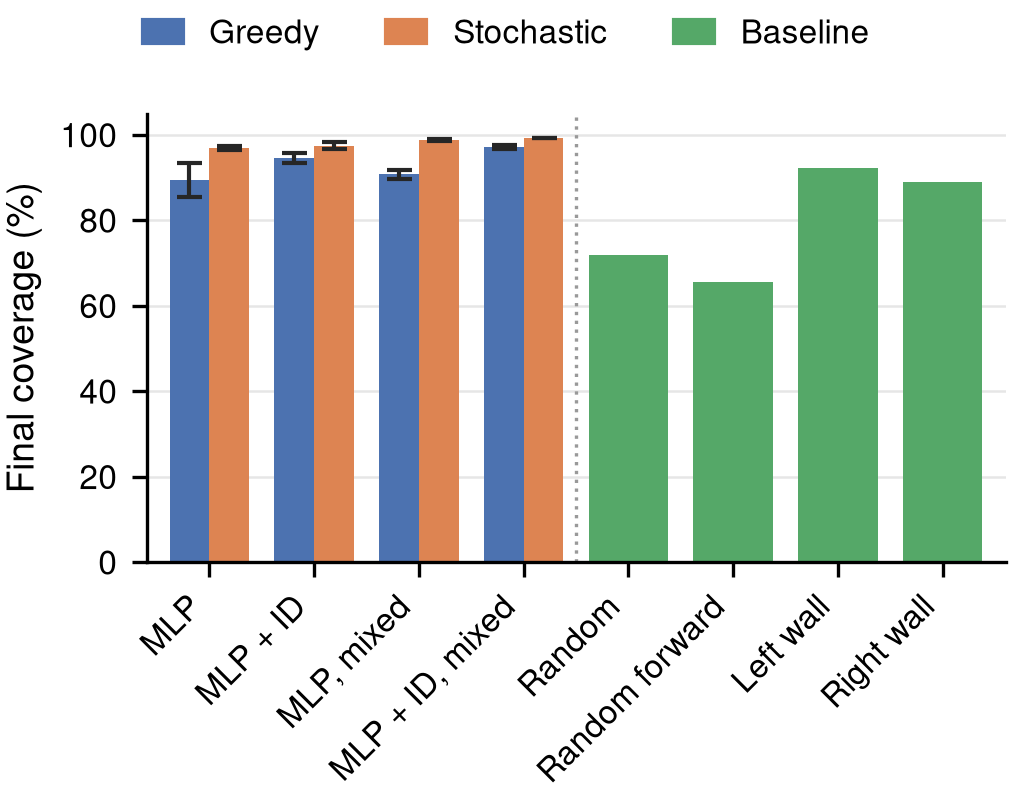
\includegraphics[width=\linewidth]{final_coverage_small}

    \small Petites cartes
    \column{0.33\textwidth}
    \centering
    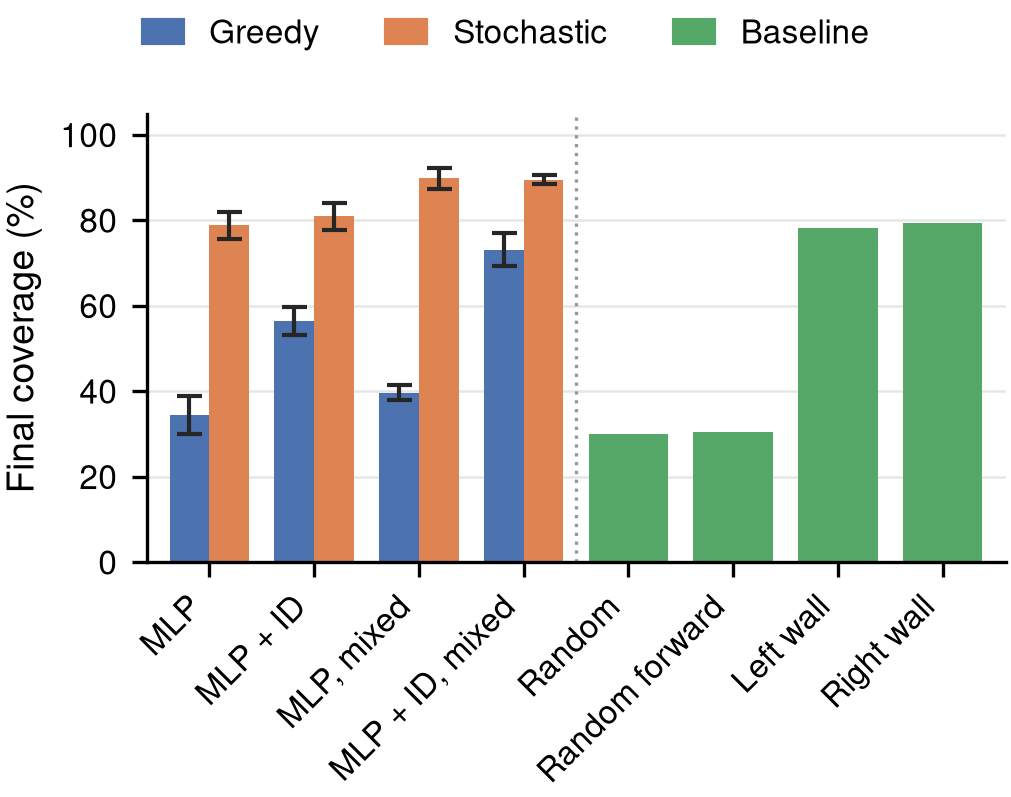
\includegraphics[width=\linewidth]{final_coverage_big}

    \small Grandes cartes
    \column{0.33\textwidth}
    \centering
    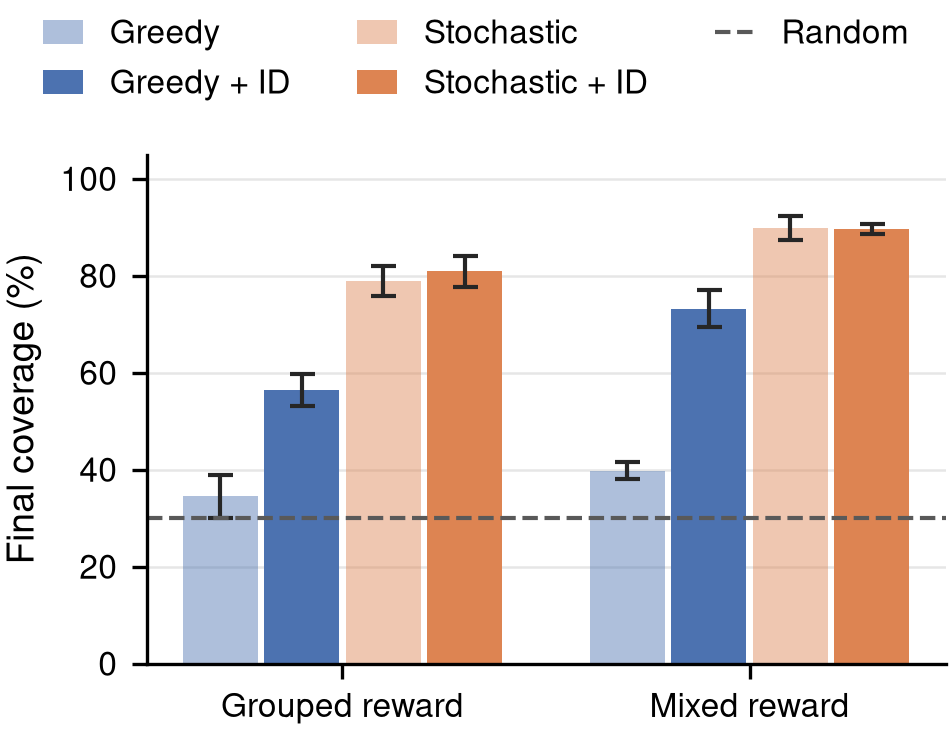
\includegraphics[width=\linewidth]{ablation_id_reward}

    \small Ablation, grandes cartes
  \end{columns}

  \vfill
  {\footnotesize Couverture finale sur \emph{val}. RL : moyenne $\pm$ écart-type sur 5 graines. Baselines : un seul run.}
\end{frame}

\begin{frame}{Simulation de la politique}
\end{frame}

\section{Case 2 : politique avec communication de signaux}

\begin{frame}{Titre}
\end{frame}

\begin{frame}{Titre}
\end{frame}

\section{Ensuite ?}

\begin{frame}{Suite du travail}
  \begin{enumerate}
    \item Entraîner les politiques à signaux pour $m = 2, 4, 6$
    \item Évaluer les baselines à carte : frontière individuelle et partagée
    \item Faire varier le nombre de drones
    \item Évaluation finale sur \emph{test}
  \end{enumerate}
\end{frame}

\end{document}
